\section{Ejercicio 5}
\subsection{Introducción}



\subsection{Resolución teórica del circuito}
Se toma el circuito propuesto por la cátedra (ver Figura \ref{fig:EQ_module})
\begin{figure}[H]
    \centering
    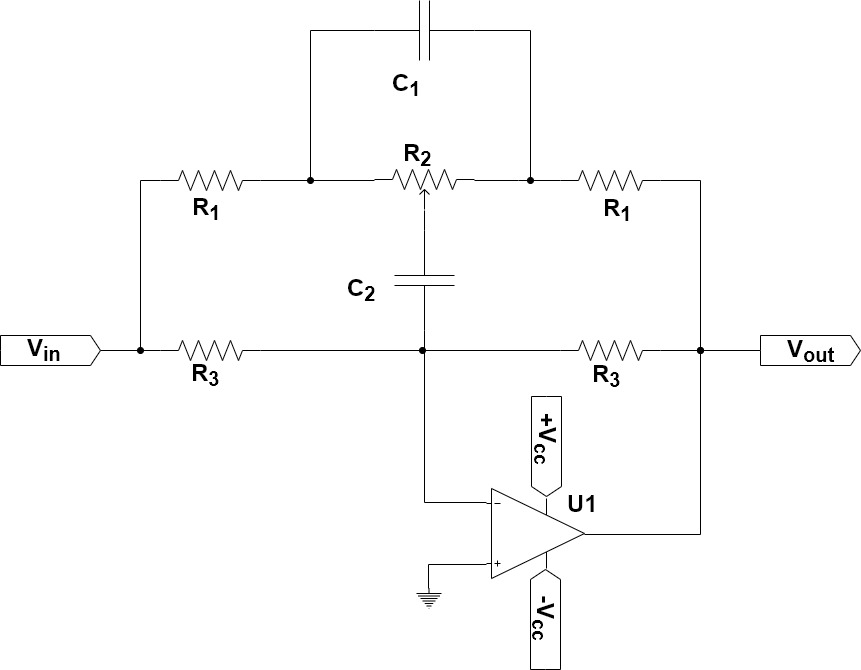
\includegraphics[width=0.6\textwidth]{../EJ5/latex_resources/EQ_module}
    \caption{Circuito ecualizador.}
    \label{fig:EQ_module}
\end{figure}

\begin{figure}[H]
    \centering
    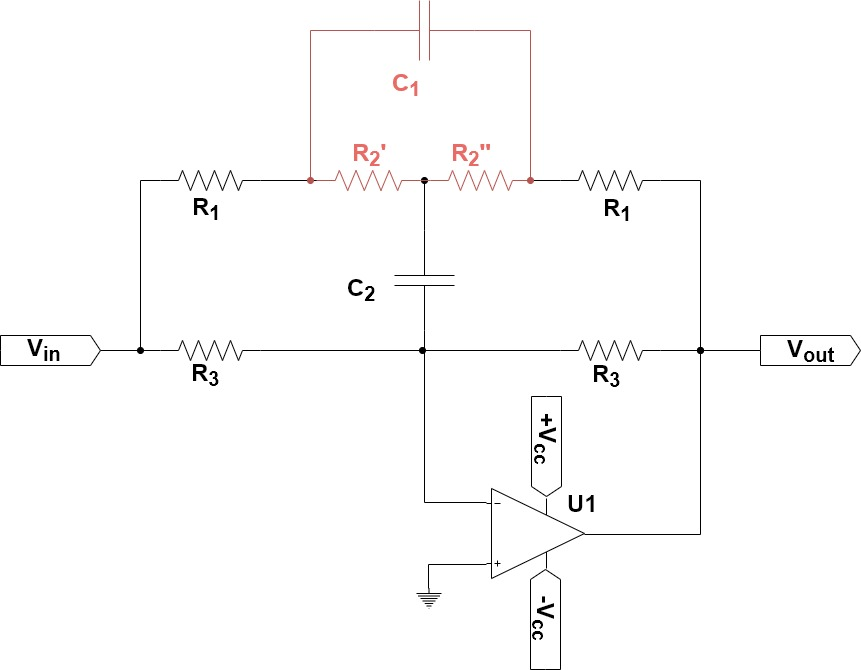
\includegraphics[width=0.6\textwidth]{../EJ5/latex_resources/Z1_2_and_3}
    \caption{Cálculo intermedio.}
    \label{fig:Z123}
\end{figure}

\begin{align}
    &Z_1 = \frac{R_2' \cdot \frac{1}{s \cdot C_1}}{R_2' + \frac{1}{s \cdot C_1} + R_2''}  \label{eq:ej5_z1} \\
    &Z_2 = \frac{R_2'' \cdot \frac{1}{s \cdot C_1}}{R_2' + \frac{1}{s \cdot C_1} + R_2''}  \label{eq:ej5_z2} \\
    &Z_3 = \frac{R_2'' \cdot R_2'}{R_2' + \frac{1}{s \cdot C_1} + R_2''}  \label{eq:ej5_z3} \\
    &R_2 = R_2' + R_2'' \label{eq:ej5_r2}
\end{align}

\begin{figure}[H]
    \centering
    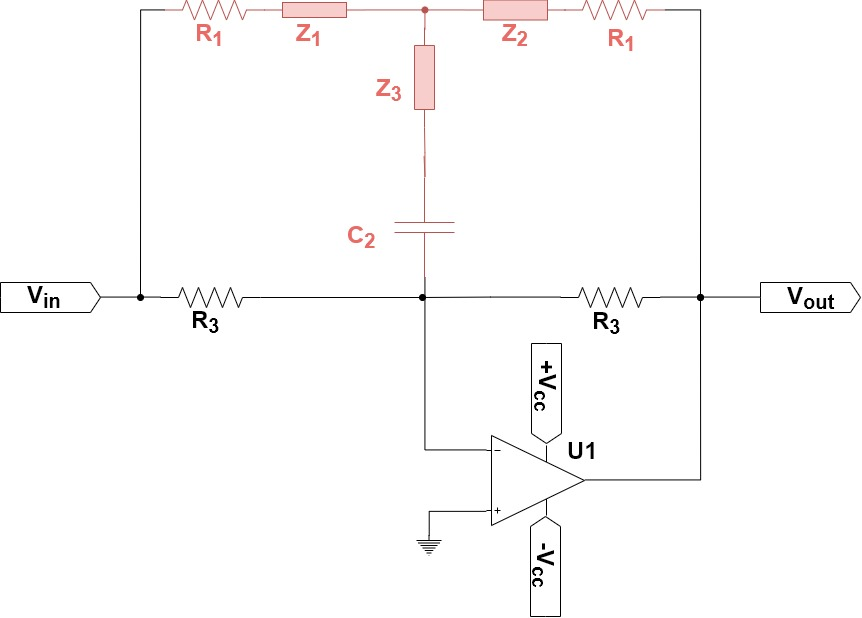
\includegraphics[width=0.6\textwidth]{../EJ5/latex_resources/Z4_5_and_6}
    \caption{Cálculo intermedio.}
    \label{fig:Z456}
\end{figure}

\begin{align}
    &Z_4 = \frac{\left(Z_1 + R_1\right) \cdot \left(Z_2 + R_1\right) + \left(Z_1 + R_1\right) \cdot \left(Z_3 + \frac{1}{s \cdot C_2}\right) + \left(Z_3 + \frac{1}{s \cdot C_2}\right) \cdot \left(Z_2 + R_1\right)}{Z_2 + R_1}  \label{eq:ej5_z4} \\
    &Z_5 = \frac{\left(Z_1 + R_1\right) \cdot \left(Z_2 + R_1\right) + \left(Z_1 + R_1\right) \cdot \left(Z_3 + \frac{1}{s \cdot C_2}\right) + \left(Z_3 + \frac{1}{s \cdot C_2}\right) \cdot \left(Z_2 + R_1\right)}{Z_3 + \frac{1}{s \cdot C_2}}  \label{eq:ej5_z5} \\
    &Z_6 = \frac{\left(Z_1 + R_1\right) \cdot \left(Z_2 + R_1\right) + \left(Z_1 + R_1\right) \cdot \left(Z_3 + \frac{1}{s \cdot C_2}\right) + \left(Z_3 + \frac{1}{s \cdot C_2}\right) \cdot \left(Z_2 + R_1\right)}{Z_1 + R_1}  \label{eq:ej5_z6}
\end{align}

\begin{figure}[H]
    \centering
    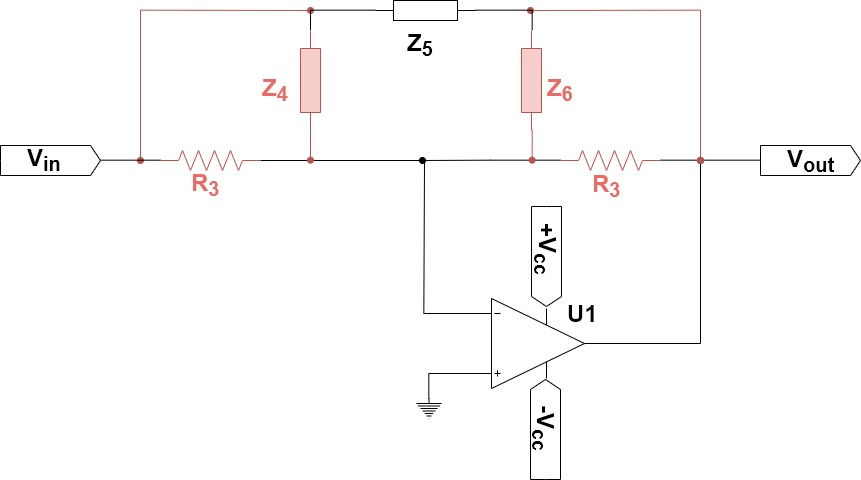
\includegraphics[width=0.6\textwidth]{../EJ5/latex_resources/Z7_and_8}
    \caption{Cálculo intermedio.}
    \label{fig:Z78}
\end{figure}

\begin{align}
    &Z_7 = \frac{R_3 \cdot Z_4}{R_3 + Z_4} \label{eq:ej5_z7} \\
    &Z_8 = \frac{R_3 \cdot Z_6}{R_3 + Z_6} \label{eq:ej5_z8}
\end{align}

\begin{align}
    &\frac{v_{out}}{v_{in}} = - \frac{Z_8}{Z_7}
\end{align}

\begin{ssmall}
\begin{adjustwidth*}{-1.3cm}{}
    \begin{align}
        &\frac{v_{out}}{v_{in}} = - \frac{C_1 \cdot C_2 \cdot R_1 \cdot \left(R_1 \cdot R_2 - 2 \cdot R_2'^2 + 2 \cdot R_2 \cdot R_2' + R_2 \cdot R_3\right) \cdot s^2 +
                                        \left(2 \cdot C_1 \cdot R_1 \cdot R_2 + C_2 \left(R_1^2 + R_1 \cdot \left(R_2 + R_3\right) - \left(R_2' + R_3\right) \cdot \left(R_2' - R_2\right)\right)\right) \cdot s +
                                        2 \cdot R_1 + R_2}
                                        {C_1 \cdot C_2 \cdot R_1 \cdot \left(R_1 \cdot R_2 - 2 \cdot R_2'^2 + 2 \cdot R_2 \cdot R_2' + R_2 \cdot R_3\right) \cdot s^2 +
                                        \left(2 \cdot C_1 \cdot R_1 \cdot R_2 + C_2 \left(R_1^2 + R_1 \cdot \left(R_2 + R_3\right) - R_2' \cdot \left(R_2' - R_2 - R_3\right)\right)\right) \cdot s +
                                        2 \cdot R_1 + R_2} \label{eq:ej5_complete_transference}
    \end{align}
\end{adjustwidth*}
\end{ssmall}

\begin{align}
    &R_3 >> R_1 \\
    &R_3 = 10 \cdot R_2 \\
    &C_1 = 10 \cdot C_2
\end{align}

\begin{align}
    &\frac{v_{out}}{v_{in}} = - \frac{\frac{20 \cdot C_2^2 \cdot R_1 \cdot \left(R_2 \cdot R_2' + 5 \cdot R_2^2 - R_2'^2\right)}{2 \cdot R_1 + R_2} \cdot s^2 +
                                        \frac{C_2 \cdot \left(30 \cdot R_1 \cdot R_2 + \left(R_2 - R_2'\right) \cdot \left(R_2' + 10 \cdot R_2\right)\right)}{2 \cdot R_1 + R_2} \cdot s +
                                        1}
                                        {\frac{20 \cdot C_2^2 \cdot R_1 \cdot \left(R_2 \cdot R_2' + 5 \cdot R_2^2 - R_2'^2\right)}{2 \cdot R_1 + R_2} \cdot s^2 +
                                        \frac{C_2 \cdot \left(31 \cdot R_1 \cdot R_2 + R_2' \cdot \left(11 \cdot R_2 - R_2'\right)\right)}{2 \cdot R_1 + R_2} \cdot s +
                                        1} \label{eq:ej5_approx_transference}
\end{align}

\begin{align}
    &f_0 = \frac{\sqrt{\frac{5 \cdot \left(2 \cdot R_1 + R_2\right)}{R_1 \cdot \left(5 \cdot R_2^2 + R_2 \cdot R_2' - R_2'^2\right)}}}{20 \pi \cdot C_2}
    \label{eq:ej5_notch_frequency}
\end{align}

Frecuencia de corte tanto para $R_2' = 0$ como para $R_2' = R_2$:
\begin{align}
    &f_0 = \frac{\sqrt{2 + \frac{R_2}{R_1}}}{20 \pi \cdot R_2 \cdot C_2}
    \label{eq:ej5_notch_frequency_limit_cases}
\end{align}

Ganancia para $s = j \cdot \omega_0$
\begin{align}
    &A_0 = - \frac{30 \cdot R_1 \cdot R_2 + \left(R_2 - R_2'\right) \cdot \left(10 \cdot R_2 + R_2'\right)}{31 \cdot R_1 \cdot R_2 + R_2' \cdot \left(11 \cdot R_2 - R_2'\right)}
    \label{eq:ej5_system_gain}
\end{align}

Ganancia para $R_2' = 0$:
\begin{align}
    &A_0 = - \frac{30 \cdot R_1 + 10 \cdot R_2}{31 \cdot R_1} \approx \frac{3 \cdot R_1 + R_2}{3 \cdot R_1}
    \label{eq:ej5_system_gain_for_R2'_0}
\end{align}

Ganancia para $R_2' = R_2$:
\begin{align}
    &A_0 = - \frac{30 \cdot R_1}{31 \cdot R_1 + 10 \cdot R_2} \approx \frac{3 \cdot R_1}{3 \cdot R_1 + R_2}
    \label{eq:ej5_system_gain_for_R2'_R2}
\end{align}



\subsection{Caracterización de polos y ceros}

\begin{figure}[H]
    \centering
    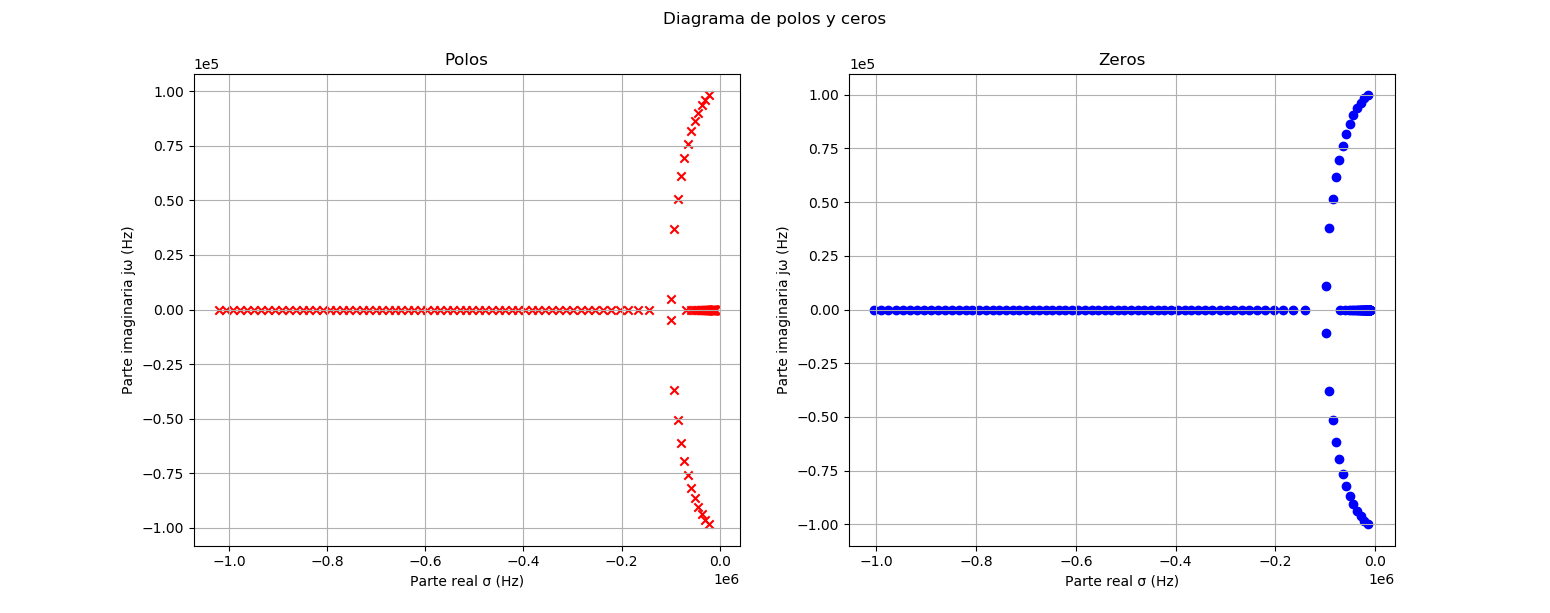
\includegraphics[width=\textwidth]{../EJ5/latex_resources/diagrama_polos_y_ceros}
    \caption{Diagramas de polos y ceros}
    \label{fig:poles_and_zeros_diag_ej5}
\end{figure}

Raíces del numerador de la transferencia aproximada:
\begin{ssmall}
\begin{align}
    &\frac{-30 \cdot R_1 + R_2 \cdot \epsilon^2 + 9 \cdot R_2 \cdot \epsilon - 10 \cdot R_2 - \sqrt{R_1^2 \cdot \left(160 \cdot \epsilon^2 - 160 \cdot \epsilon + 100\right) + R_1 \cdot R_2 \cdot \left(20 \cdot \epsilon^2 - 620 \cdot \epsilon + 200\right) + R_2^2 \cdot \left(\epsilon^4 + 18 \cdot \epsilon^3 + 61 \cdot \epsilon^2 - 180 \cdot \epsilon + 100\right)}}{40 \cdot C_2 \cdot R_1 \cdot R_2 \cdot (-\epsilon^2 + \epsilon + 5)} \\
    &\frac{-30 \cdot R_1 + R_2 \cdot \epsilon^2 + 9 \cdot R_2 \cdot \epsilon - 10 \cdot R_2 + \sqrt{R_1^2 \cdot \left(160 \cdot \epsilon^2 - 160 \cdot \epsilon + 100\right) + R_1 \cdot R_2 \cdot \left(20 \cdot \epsilon^2 - 620 \cdot \epsilon + 200\right) + R_2^2 \cdot \left(\epsilon^4 + 18 \cdot \epsilon^3 + 61 \cdot \epsilon^2 - 180 \cdot \epsilon + 100\right)}}{40 \cdot C_2 \cdot R_1 \cdot R_2 \cdot (-\epsilon^2 + \epsilon + 5)} 
    \label{eq:ej5_num_roots_simplyfied_system}
\end{align}
\end{ssmall}

%Raíces del numerador de la transferencia completa:
%\begin{ssmall}
%\begin{align}
%    \frac{-R_1^2 - 31 \cdot R_1 \cdot R_2 + R_2^2 \cdot \epsilon^2 + 9 \cdot R_2^2 \cdot \epsilon - 10 \cdot R_2^2 - \sqrt{R_1^4 - 18 \cdot R_1^3 \cdot R_2 + 158 \cdot R_1^2 \cdot R_2^2 \cdot \epsilon^2 - 178 \cdot R_1^2 \cdot R_2^2 \cdot \epsilon + 141 \cdot R_1^2 \cdot R_2^2 + 18 \cdot R_1 \cdot R_2^3 \cdot \epsilon^2 - 638 \cdot R_1 \cdot R_2^3 \cdot \epsilon + 220 \cdot R_1 \cdot R_2^3 + R_2^4 \cdot \epsilon^4 + 18 \cdot R_2^4 \cdot \epsilon^3 + 61 \cdot R_2^4 \cdot \epsilon^2 - 180 \cdot R_2^4 \cdot \epsilon + 100 \cdot R_2^4}}{20 \cdot C_2 \cdot R_1 \cdot R_2 \cdot (R_1 - 2 \cdot R_2 \cdot \epsilon^2 + 2 \cdot R_2 \cdot \epsilon + 10 \cdot R_2} \\
%    \frac{-R_1^2 - 31 \cdot R_1 \cdot R_2 + R_2^2 \cdot \epsilon^2 + 9 \cdot R_2^2 \cdot \epsilon - 10 \cdot R_2^2 + \sqrt{R_1^4 - 18 \cdot R_1^3 \cdot R_2 + 158 \cdot R_1^2 \cdot R_2^2 \cdot \epsilon^2 - 178 \cdot R_1^2 \cdot R_2^2 \cdot \epsilon + 141 \cdot R_1^2 \cdot R_2^2 + 18 \cdot R_1 \cdot R_2^3 \cdot \epsilon^2 - 638 \cdot R_1 \cdot R_2^3 \cdot \epsilon + 220 \cdot R_1 \cdot R_2^3 + R_2^4 \cdot \epsilon^4 + 18 \cdot R_2^4 \cdot \epsilon^3 + 61 \cdot R_2^4 \cdot \epsilon^2 - 180 \cdot R_2^4 \cdot \epsilon + 100 \cdot R_2^4}}{20 \cdot C_2 \cdot R_1 \cdot R_2 \cdot (R_1 - 2 \cdot R_2 \cdot \epsilon^2 + 2 \cdot R_2 \cdot \epsilon + 10 \cdot R_2}
%    \label{eq:ej5_num_root}
%\end{align}
%\end{ssmall}

Intento cambiando parte real del numerador:
\begin{align}
    &-30 \cdot R_1 + R_2 \cdot \epsilon^2 + 9 \cdot \epsilon - 10 \cdot R_2 > 0
    \label{eq:ej5_attempting_changing_zeros_with_real_part}
\end{align}

Resultado de intentar cambiar parte real del numerador con $\epsilon = 0$:
\begin{align}
    &R_1 < -\frac{1}{3} \cdot R_2
    \label{eq:ej5_results_of_attempting_changing_zeros_with_real_part_epsilon_0}
\end{align}

Resultado de intentar cambiar parte real del numerador con $\epsilon = 1$:
\begin{align}
    &R_1 < 0
    \label{eq:ej5_results_of_attempting_changing_zeros_with_real_part_epsilon_1}
\end{align}

Intento haciendo que el modulo de la parte con raíz sea mayor al de la parte sin:
\begin{ssmall}
\begin{align}
    \left|-30 \cdot R_1 + R_2 \cdot \epsilon^2 + 9 \cdot \epsilon - 10 \cdot R_2 \right| < \left|\sqrt{R_1^2 \cdot \left(160 \cdot \epsilon^2 - 160 \cdot \epsilon + 100\right) + R_1 \cdot R_2 \cdot \left(20 \cdot \epsilon^2 - 620 \cdot \epsilon + 200\right) + R_2^2 \cdot \left(\epsilon^4 + 18 \cdot \epsilon^3 + 61 \cdot \epsilon^2 - 180 \cdot \epsilon + 100\right)}\right|
    \label{eq:ej5_attempting_changing_zeros_with_root}
\end{align}
\end{ssmall}

Resultado de intentar cambiar con modulo de la raíz para $\epsilon = 0$:
\begin{align}
    &3 \cdot R_1 + R_2 < R_1 + R_2
    \label{eq:ej5_results_of_attempting_changing_zeros_with_root_epsilon_0}
\end{align}

Resultado de intentar cambiar con modulo de la raíz para $\epsilon = 1$:
\begin{align}
    &800 \cdot R_1 < -4 \cdot R_2
    \label{eq:ej5_results_of_attempting_changing_zeros_with_root_epsilon_1}
\end{align}



\subsection{Diseño de ecualizador de 3 bandas}
Las frecuencias para las 3 bandas, usando \ref{eq:ej5_notch_frequency_limit_cases}:
\begin{align}
    &f_{01} = \frac{\sqrt{2 + \frac{10 K\Omega}{10\Omega}}}{20\pi \cdot 10 K\Omega \cdot 390 nF} = 129.2 Hz \\
    &f_{02}= \frac{\sqrt{2 + \frac{1 K\Omega}{10\Omega}}}{20\pi \cdot 1 K\Omega \cdot 150 nF} = 1.072 KHz \\
    &f_{03} = \frac{\sqrt{2 + \frac{1 K\Omega}{10\Omega}}}{20\pi \cdot 1 K\Omega \cdot 22 nF} = 7.306 KHz
\end{align}

\todo[inline]{Show why I have to put them in cascade and not as a mixer}